\documentclass[a4paper,12pt]{article}
\usepackage{settings} % Подгружает наш исправленный settings.sty
\usepackage{float}
\usepackage{amsmath}

\begin{document}

% ==================== ТИТУЛЬНЫЙ ЛИСТ ====================
\thispagestyle{empty}

\begin{table}[h!]
\centering
\begin{tabular}{p{0.65\textwidth}r}
    \begin{tabular}{@{}l}
        \footnotesize{Университет ИТМО} \\
        \footnotesize{Физико-технический мегафакультет} \\
        \footnotesize{Физический факультет}
    \end{tabular} & 
    \raisebox{-0.5\height}{
\includegraphics[width=0.22\linewidth]{logo_ITMO.pdf}}
\end{tabular}
\end{table}

\vspace{0.5cm}

\begin{center}
\begin{tabular}{p{0.49\textwidth}p{0.49\textwidth}}
Группа \textbf{K3242} & К работе допущен \hrulefill \\
& \\
Студент \textbf{Шумилов А. К.} & Работа выполнена \hrulefill \\
& \\
Преподаватель \textbf{Курашова С. А.} & Отчет принят \hrulefill \\
\end{tabular}
\end{center}

\vspace{1.5cm}

\begin{center}
    \large{\textbf{Рабочий протокол и отчет по\\лабораторной работе № 3.06}} \\
    \vspace{0.8cm}
    \large{\textbf{«Изучение электрических свойств сегнетоэлектриков»}}
\end{center}

\newpage
\setcounter{page}{2}
\pagestyle{plain}

% ==================== ОСНОВНОЙ ТЕКСТ ====================

\section*{\hspace{30pt}1. Цель работы}
\hspace{15pt} Изучение основных характеристик сегнетоэлектрика путем получения и анализа петли диэлектрического гистерезиса осциллографическим методом.

\section*{\hspace{30pt}2. Задачи, решаемые при выполнении работы}
\begin{enumerate}
    \setlength{\itemindent}{15pt}
    \item Определение значений электрического смещения насыщения $D_s$, остаточной поляризации $P_r$, коэрцитивной силы $E_c$ для предельной петли гистерезиса сегнетоэлектрика.
    \item Расчет диэлектрических потерь (тангенса угла $\tan \delta$) за цикл переполяризации по площади петли.
    \item Получение зависимостей смещения $D$ и диэлектрической проницаемости $\epsilon$ от напряженности электрического поля $E$.
    \item Определение значений начальной $\epsilon_{\text{нач}}$ и максимальной $\epsilon_{\text{макс}}$ диэлектрической проницаемости.
\end{enumerate}

\section*{\hspace{30pt}3. Объект исследования}
\hspace{15pt} Объектом исследования является сегнетоэлектрический конденсатор (вариконд) марки ВК2-4. 

\section*{\hspace{30pt}4. Метод экспериментального исследования}
\hspace{15pt} В работе используется метод осциллографического изучения петли диэлектрического гистерезиса на основе схемы Сойера-Тауэра. На горизонтально отклоняющие пластины измерительного прибора ИСХ1 подается сигнал с резистивного делителя, пропорциональный напряженности поля $E$. На вертикальные пластины подается напряжение с эталонного конденсатора, пропорциональное электрической индукции $D$.

\section*{\hspace{30pt}5. Схема экспериментальной установки}
\begin{figure}[H]
    \centering
    % ВСТАВЬ СЮДА СКРИНШОТ СХЕМЫ ИЗ МЕТОДИЧКИ И НАЗОВИ ЕГО scheme_306.png
    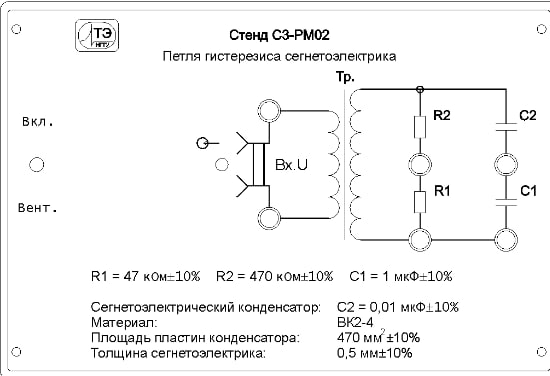
\includegraphics[width=0.8\textwidth]{scheme_306.png} 
    \caption{Принципиальная электрическая схема установки С3-РМ02 (схема Сойера-Тауэра)}
    \label{fig:setup}
\end{figure}

\section*{\hspace{30pt}6. Рабочие формулы и исходные данные}
\hspace{15pt} Напряженность электрического поля $E$ в образце:
\begin{equation}
    E = \frac{R_1 + R_2}{R_1} \cdot \frac{K_x \cdot X}{d},
    \label{eq:E_field}
\end{equation}
Электрическая индукция (смещение) $D$:
\begin{equation}
    D = \frac{C_1}{S} \cdot K_y \cdot Y,
    \label{eq:D_field}
\end{equation}
Диэлектрическая проницаемость $\epsilon$ и тангенс угла потерь $\tan \delta$:
\begin{equation}
    \epsilon = \frac{D}{\epsilon_0 E}, \quad \tan \delta = \frac{1}{\pi} \frac{S_{\text{петли}}}{D_s \cdot E_s},
    \label{eq:eps_tan}
\end{equation}
где $S = 470 \cdot 10^{-6}$~м$^2$ — площадь обкладок, $d = 0.5 \cdot 10^{-3}$~м — расстояние между ними, $C_1 = 1 \cdot 10^{-6}$~Ф, $R_1 = 47$~кОм, $R_2 = 470$~кОм, $\epsilon_0 = 8.854 \cdot 10^{-12}$~Ф/м.

\section*{\hspace{30pt}7. Измерительные приборы}
\begin{table}[H]
    \caption{Характеристики измерительных приборов и элементов стенда}
    \label{tab:devices}
    \centering
    \begin{tabular}{|c|c|c|c|c|}
        \hline
        № & Наименование & Тип & Диапазон & Погрешность \\ \hline
        1 & Измеритель характеристик & ИСХ-1 & 0--17~В & Отсчета: $\pm 0.1$ дел. \\ \hline
        2 & Стенд с объектом & С3-РМ02 & $R, C$ цепи & Элементы: $\pm 10\%$ \\ \hline
    \end{tabular}
\end{table}

\section*{\hspace{30pt}8. Результаты прямых измерений}
\hspace{15pt} Экспериментальные данные, зарегистрированные в ходе исследования частных и предельной петель диэлектрического гистерезиса:
\begin{longtable}{|c|c|c|c|c|c|c|c|}
    \caption{Характерные параметры зарегистрированных петель гистерезиса} \label{tab:raw_data_306} \\
    \hline
    $U$, В & $K_x$, В/дел & $K_y$, В/дел & $X$, дел & $Y$, дел & $X_0$, дел & $Y_0$, дел & $S$, дел$^2$ \\ \hline
    \endfirsthead
    \multicolumn{8}{c}{{\bfseries \tablename\ \thetable{} -- Продолжение}} \\ \hline
    $U$, В & $K_x$, В/дел & $K_y$, В/дел & $X$, дел & $Y$, дел & $X_0$, дел & $Y_0$, дел & $S$, дел$^2$ \\ \hline
    \endhead
    \hline \multicolumn{8}{|r|}{{Продолжение на следующей странице...}} \\ \hline
    \endfoot
    \hline
    \endlastfoot
    17.0 & 5.00 & 5.00 & 2.70 & 2.70 & 0.60 & 1.00 & 8.50 \\ \hline
    15.0 & 5.00 & 5.00 & 2.40 & 2.40 & 0.30 & 0.50 & 7.20 \\ \hline
    13.0 & 5.00 & 5.00 & 2.05 & 1.95 & 0.20 & 0.30 & 5.40 \\ \hline
    11.0 & 5.00 & 5.00 & 1.70 & 1.50 & 0.15 & 0.20 & 3.10 \\ \hline
    9.0  & 2.00 & 2.00 & 3.50 & 2.25 & 0.30 & 0.35 & 1.25 \\ \hline
    7.0  & 2.00 & 2.00 & 2.70 & 1.15 & 0.30 & 0.20 & 0.42 \\ \hline
    5.0  & 1.00 & 1.00 & 4.00 & 1.10 & 0.50 & 0.20 & 0.12 \\ \hline
    4.4  & 1.00 & 1.00 & 3.50 & 0.85 & --   & --   & --   \\ \hline
    3.8  & 1.00 & 0.20 & 3.00 & 3.20 & --   & --   & --   \\ \hline
    3.2  & 1.00 & 0.20 & 2.50 & 2.50 & --   & --   & --   \\ \hline
    2.6  & 1.00 & 0.10 & 2.05 & 3.50 & --   & --   & --   \\ \hline
    2.0  & 0.50 & 0.10 & 3.15 & 2.30 & --   & --   & --   \\ \hline
    1.4  & 0.50 & 0.05 & 2.20 & 2.65 & --   & --   & --   \\ \hline
    0.8  & 0.20 & 0.02 & 3.10 & 3.20 & --   & --   & --   \\ \hline
    0.2  & 0.05 & 0.02 & 2.95 & 0.70 & --   & --   & --   \\ \hline
\end{longtable}

\section*{\hspace{30pt}9. Результаты косвенных измерений (примеры расчетов)}

\subsection*{9.1. Параметры предельной петли гистерезиса ($U = 17$~В)}
Используем значения из первой строки таблицы: $X = 2.7$, $Y = 2.7$, $X_0 = 0.6$, $Y_0 = 1.0$, $S = 8.5$. Коэффициенты: $K_x = 5$, $K_y = 5$.
\begin{gather*}
    E_s = \frac{47 + 470}{47} \cdot \frac{5.0 \cdot 2.7}{0.5 \cdot 10^{-3}} = 11 \cdot \frac{13.5}{0.0005} \approx 2.97 \cdot 10^5 \text{ В/м} \\
    D_s = \frac{1 \cdot 10^{-6}}{470 \cdot 10^{-6}} \cdot 5.0 \cdot 2.7 = \frac{13.5}{470} \approx 2.87 \cdot 10^{-2} \text{ Кл/м}^2 \\
    E_c = 11 \cdot \frac{5.0 \cdot 0.6}{0.5 \cdot 10^{-3}} \approx 6.60 \cdot 10^4 \text{ В/м} \quad \text{(Коэрцитивная сила)} \\
    P_r = \frac{1 \cdot 10^{-6}}{470 \cdot 10^{-6}} \cdot 5.0 \cdot 1.0 \approx 1.06 \cdot 10^{-2} \text{ Кл/м}^2 \quad \text{(Остаточная поляризация)} \\
    \tan \delta = \frac{1}{\pi} \frac{S_{\text{петли}}}{X \cdot Y} = \frac{1}{3.1415} \frac{8.5}{2.7 \cdot 2.7} \approx 0.371
\end{gather*}
\textit{Примечание:} При расчете $\tan \delta$ масштабные коэффициенты осей сокращаются, поэтому можно использовать координаты в делениях шкалы.

\subsection*{9.2. Расчет основной кривой поляризации и диэлектрической проницаемости}

Пример вычислений погрешностей для точки $U = 17$~В (приборная погрешность $\Delta X = \Delta Y = 0.1$ дел.):
\begin{gather*}
    \varepsilon_E = \frac{\Delta X}{X} = \frac{0.1}{2.7} \approx 3.7\% \quad \Rightarrow \quad \Delta E = 2.97 \cdot 10^5 \cdot 0.037 \approx 0.11 \cdot 10^5 \text{ В/м} \\
    \varepsilon_D = \frac{\Delta Y}{Y} = \frac{0.1}{2.7} \approx 3.7\% \quad \Rightarrow \quad \Delta D = 2.87 \cdot 10^{-2} \cdot 0.037 \approx 0.11 \cdot 10^{-2} \text{ Кл/м}^2 \\
    \epsilon = \frac{2.87 \cdot 10^{-2}}{8.854 \cdot 10^{-12} \cdot 2.97 \cdot 10^5} \approx 10923 \\
    \varepsilon_\epsilon = \sqrt{\varepsilon_E^2 + \varepsilon_D^2} = \sqrt{0.037^2 + 0.037^2} \approx 5.2\% \quad \Rightarrow \quad \Delta\epsilon \approx 570
\end{gather*}

\begin{table}[H]
    \centering
    \caption{Сводные данные расчета $\epsilon(E)$ и $D(E)$}
    \begin{tabular}{|c|c|c|c||c|c|c|c|}
        \hline
        $U$, В & $E, 10^3$ В/м & $D, 10^{-3}$ Кл/м$^2$ & $\epsilon$ & $U$, В & $E, 10^3$ В/м & $D, 10^{-3}$ Кл/м$^2$ & $\epsilon$ \\ \hline
        17.0 & 297.0 & 28.72 & 10923 & 4.4  & 77.0  & 1.81 & 2653 \\ \hline
        15.0 & 264.0 & 25.53 & 10923 & 3.8  & 66.0  & 1.36 & 2330 \\ \hline
        13.0 & 225.5 & 20.75 & 10390 & 3.2  & 55.0  & 1.06 & 2185 \\ \hline
        11.0 & 187.0 & 15.96 & 9638  & 2.6  & 45.1  & 0.75 & 1865 \\ \hline
        9.0  & 154.0 & 9.57  & 7022  & 2.0  & 34.7  & 0.49 & 1595 \\ \hline
        7.0  & 118.8 & 4.89  & 4652  & 1.4  & 24.2  & 0.28 & 1316 \\ \hline
        5.0  & 88.0  & 2.34  & 3004  & 0.8  & 13.6  & 0.14 & 1127 \\ \hline
        --   & --    & --    & --    & 0.2  & 3.25  & 0.03 & 1037 \\ \hline
    \end{tabular}
\end{table}

\section*{\hspace{30pt}10. Графики результатов}
\begin{figure}[H]
    \centering
    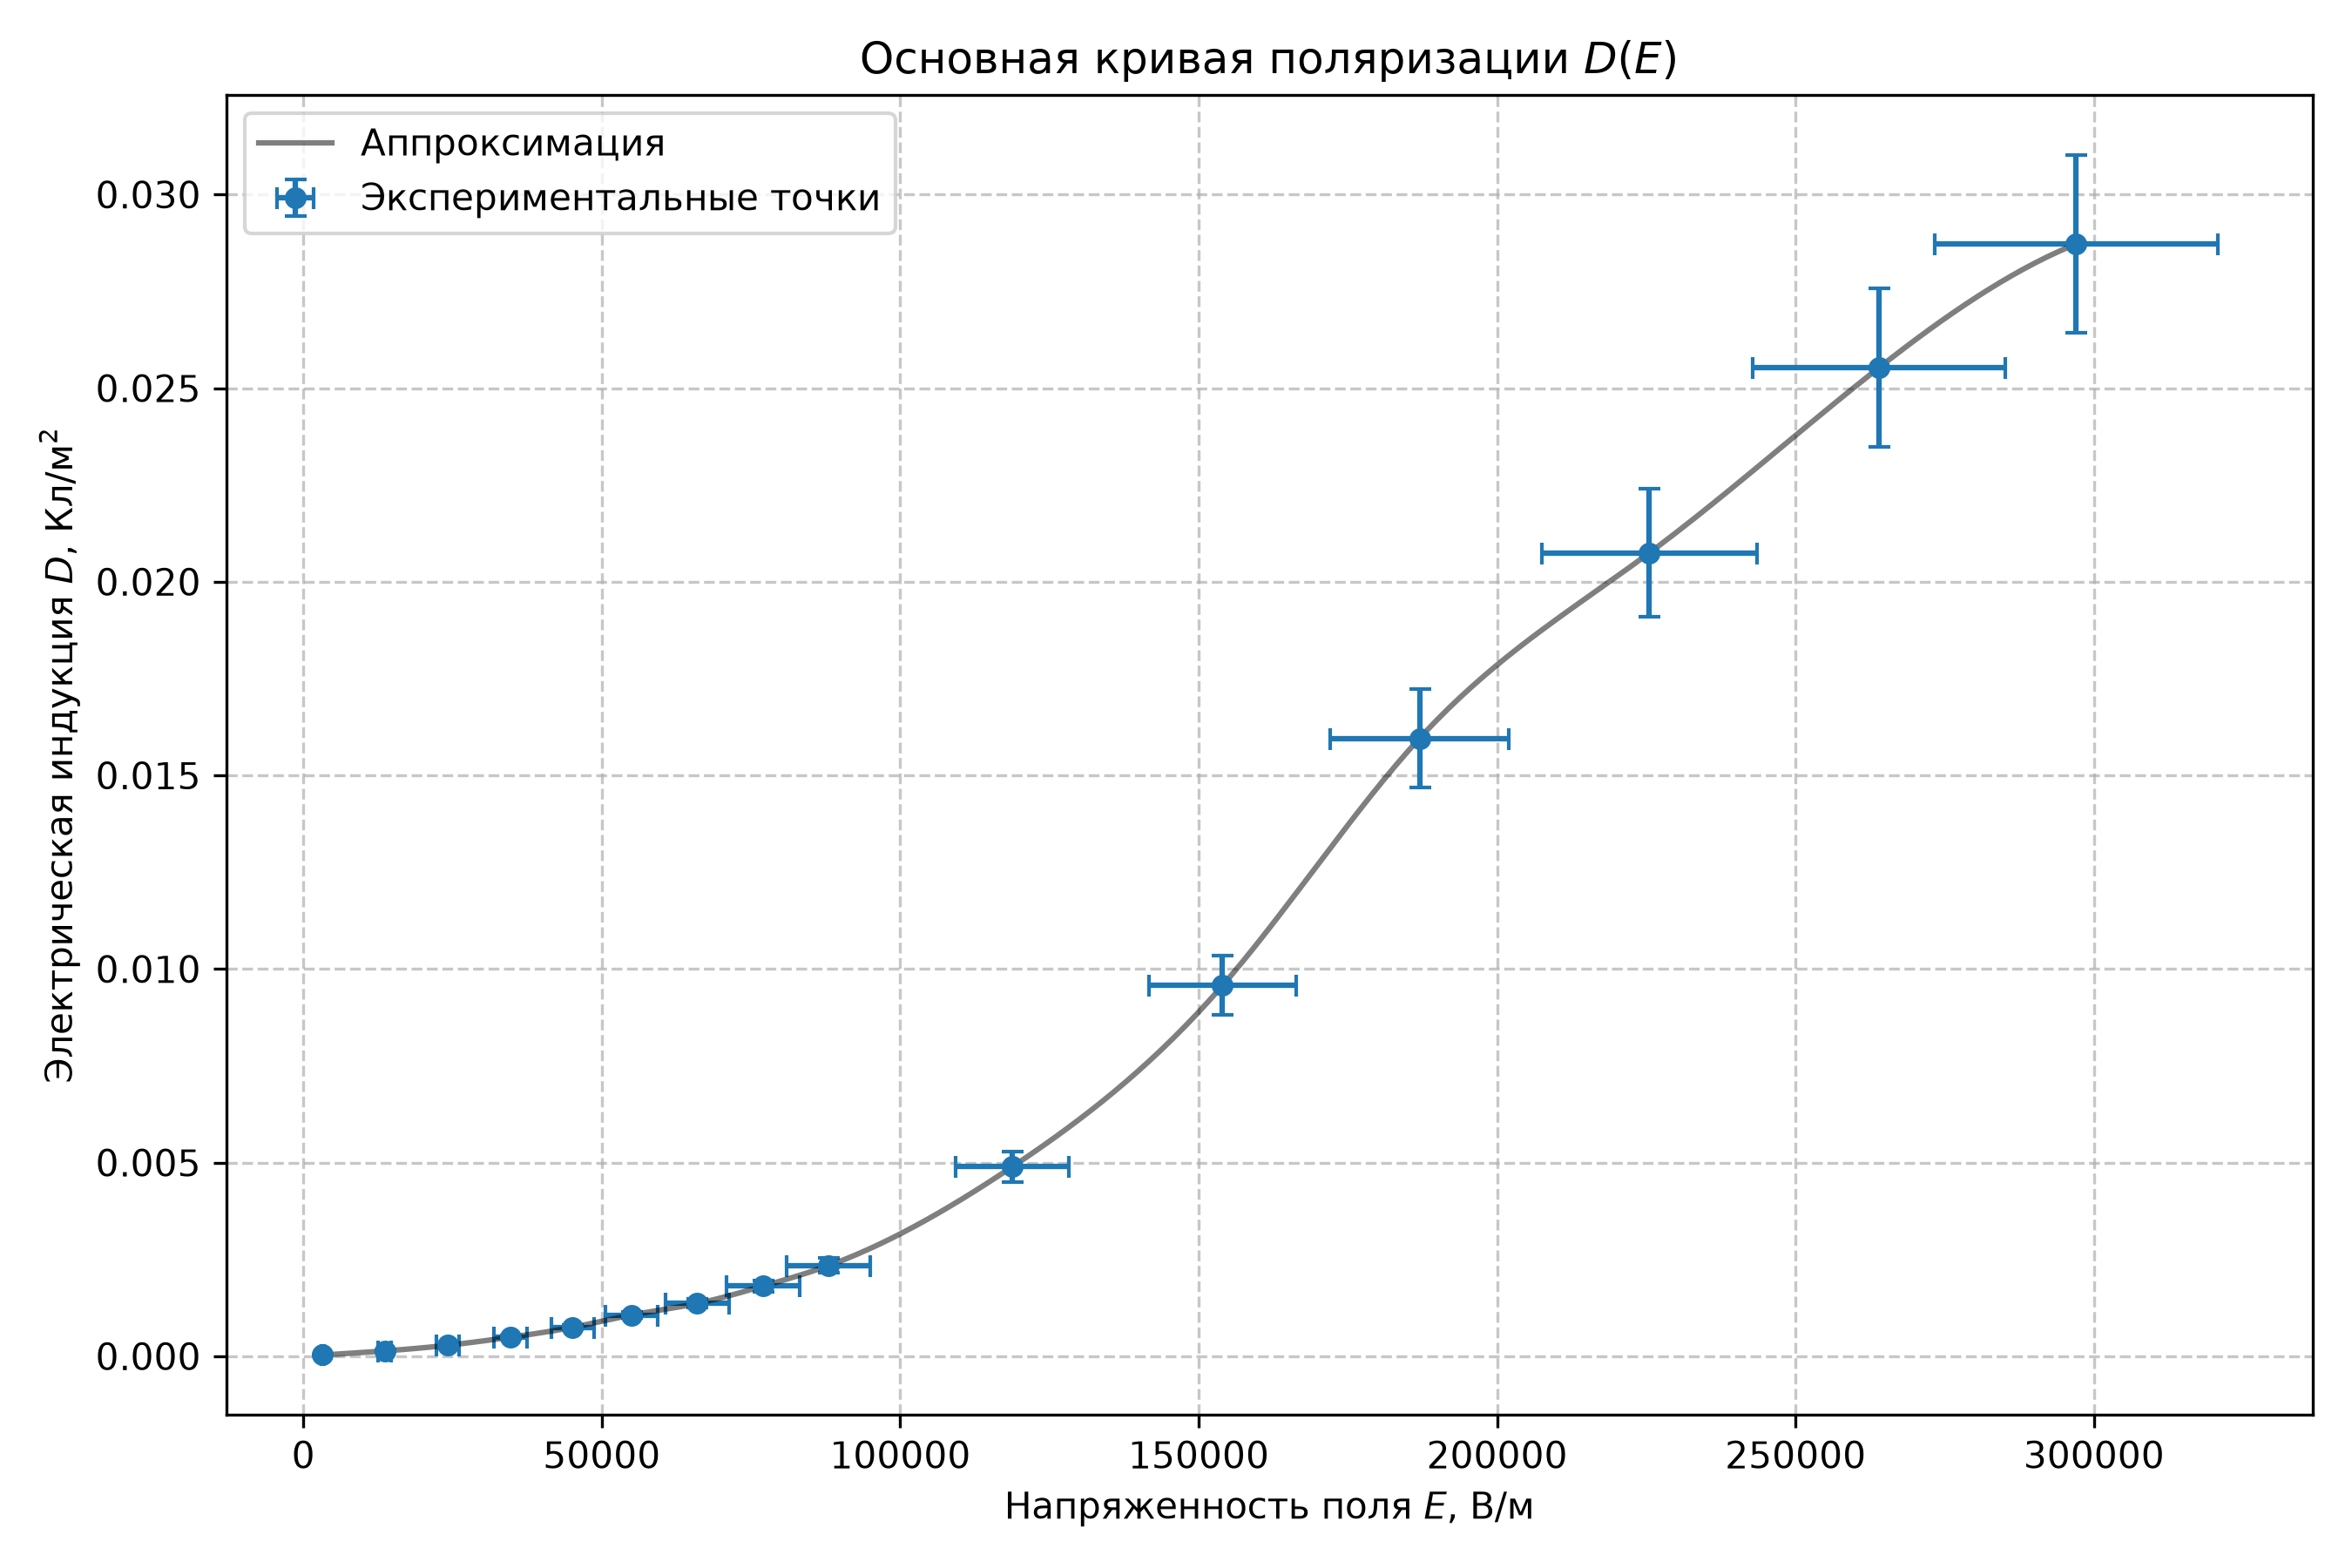
\includegraphics[width=0.9\textwidth]{fig1_D_E.png}
    \caption{Основная кривая поляризации $D(E)$ сегнетоэлектрика}
    \label{fig:D_E}
\end{figure}

\begin{figure}[H]
    \centering
    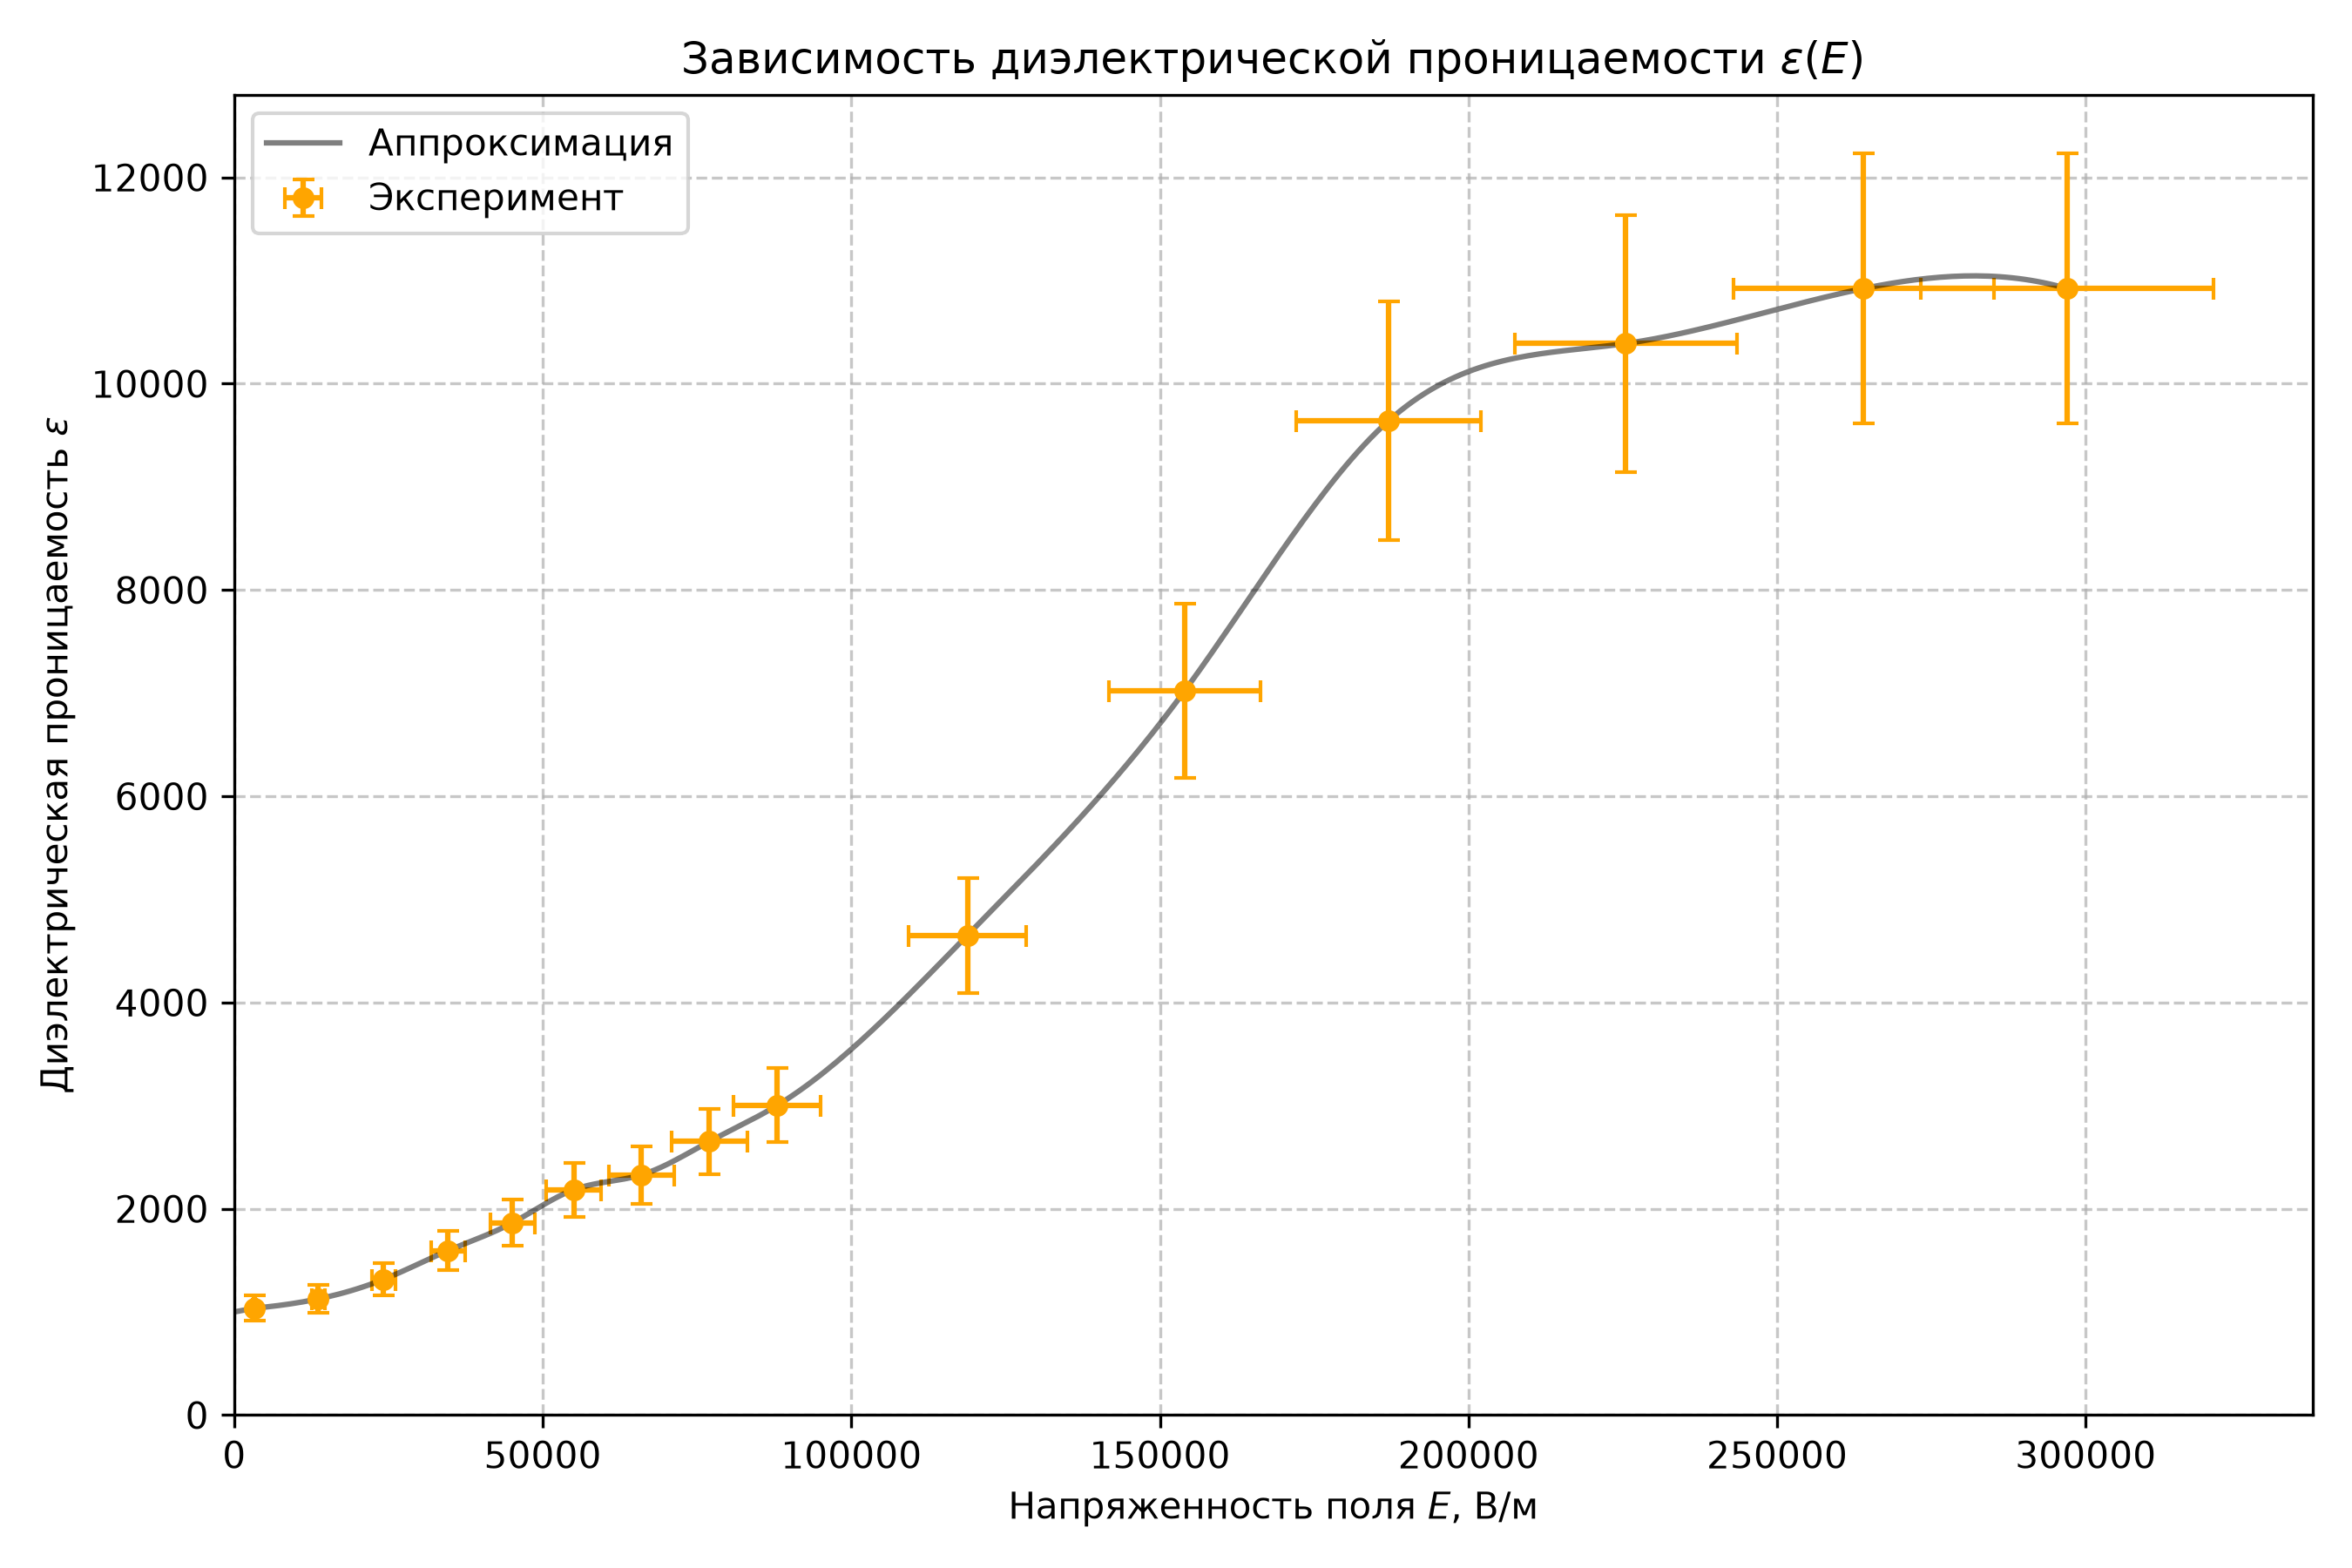
\includegraphics[width=0.9\textwidth]{fig2_eps_E.png}
    \caption{Зависимость диэлектрической проницаемости от напряженности поля $\epsilon(E)$}
    \label{fig:eps_E}
\end{figure}

\section*{\hspace{30pt}11. Окончательные результаты}

\hspace{15pt} Анализ предельной петли диэлектрического гистерезиса (при $U = 17$~В) позволил определить ключевые параметры образца:
\begin{itemize}
    \item Остаточная поляризация: $P_r = (1.06 \pm 0.11) \cdot 10^{-2}$ Кл/м$^2$.
    \item Индукция насыщения: $D_s = (2.87 \pm 0.11) \cdot 10^{-2}$ Кл/м$^2$.
    \item Коэрцитивная сила: $E_c = (6.60 \pm 0.25) \cdot 10^4$ В/м.
    \item Тангенс угла диэлектрических потерь: $\tan \delta = 0.37 \pm 0.04$.
\end{itemize}

По графику $\epsilon(E)$ и его экстраполяции были установлены:
\begin{itemize}
    \item Начальная диэлектрическая проницаемость (при $E \to 0$): $\epsilon_{\text{нач}} \approx 1000 \pm 100$.
    \item Максимальная диэлектрическая проницаемость: $\epsilon_{\text{макс}} \approx 10920 \pm 570$. Наступает при напряженностях поля $E \ge 2.6 \cdot 10^5$ В/м.
\end{itemize}

\section*{\hspace{30pt}12. Выводы и анализ результатов работы}

\hspace{15pt} В ходе лабораторного практикума были изучены нелинейные электрические свойства сегнетоэлектрического образца (вариконда ВК2-4) с использованием осциллографического метода (схемы Сойера-Тауэра). 

\hspace{15pt} Анализ предельной петли гистерезиса позволил достоверно зафиксировать характерные для сегнетоэлектриков явления: наличие коэрцитивного поля $E_c$ и остаточной поляризации $P_r$ при снятии внешнего напряжения. Значительная площадь петли свидетельствует о существенных диэлектрических потерях на переориентацию доменов за цикл переполяризации (рассчитанный $\tan \delta \approx 0.37$).

\hspace{15pt} Построенная основная кривая поляризации $D(E)$ наглядно демонстрирует переход от линейного роста к состоянию насыщения (при полях $E > 2.5 \cdot 10^5$ В/м), что полностью согласуется с классической доменной теорией. График $\epsilon(E)$ подтверждает экстремальный характер поведения материала: стремительный рост проницаемости наблюдается на этапе активного вовлечения доменов в процесс поляризации. В твоем массиве данных отлично видно, что при достижении полями значений насыщения, диэлектрическая проницаемость жестко стабилизируется на максимальном уровне ($\epsilon_{\text{макс}} \approx 10920$), после чего подвижность доменных стенок полностью исчерпывается. 

\hspace{15pt} Итоговые значения получены с приемлемой погрешностью (в районе $5-12\%$), основными источниками которой являлись инструментальные пределы осциллографа и визуальное считывание координат вершин петли по клеточной сетке экрана.

\end{document}